\documentclass[11pt,a4paper]{article}
\usepackage{titlesec}
\usepackage[latin1]{inputenc}
\usepackage{geometry}
%\usepackage{showframe} %This line can be used to clearly show the new margins
\newgeometry{vmargin={15mm}, hmargin={18mm,18mm}}   % set the margins
\usepackage{subcaption}
\usepackage{amsmath}
\usepackage{amsfonts}
\usepackage{amssymb}
\usepackage{graphicx}
\usepackage{tikz}
\usepackage{hyperref}
\usetikzlibrary{intersections}
\author{Jama Hussein Mohamud}
\title{Object Tracker}
\begin{document}
\maketitle
\titlespacing*{\section}{0pt}{1.1\baselineskip}{\baselineskip}
\section{Introduction}
Object tracking has been a long-term goal in computer vision and this project will focus on implementing an object tracking system by estimating the trajectory of objects in a sequence of consecutive frames. The idea will be to calculate the Euclidean distance between objects in subsequent frames. \\

\begin{figure}[!h]
\centering
\begin{subfigure}[b]{0.48\textwidth}
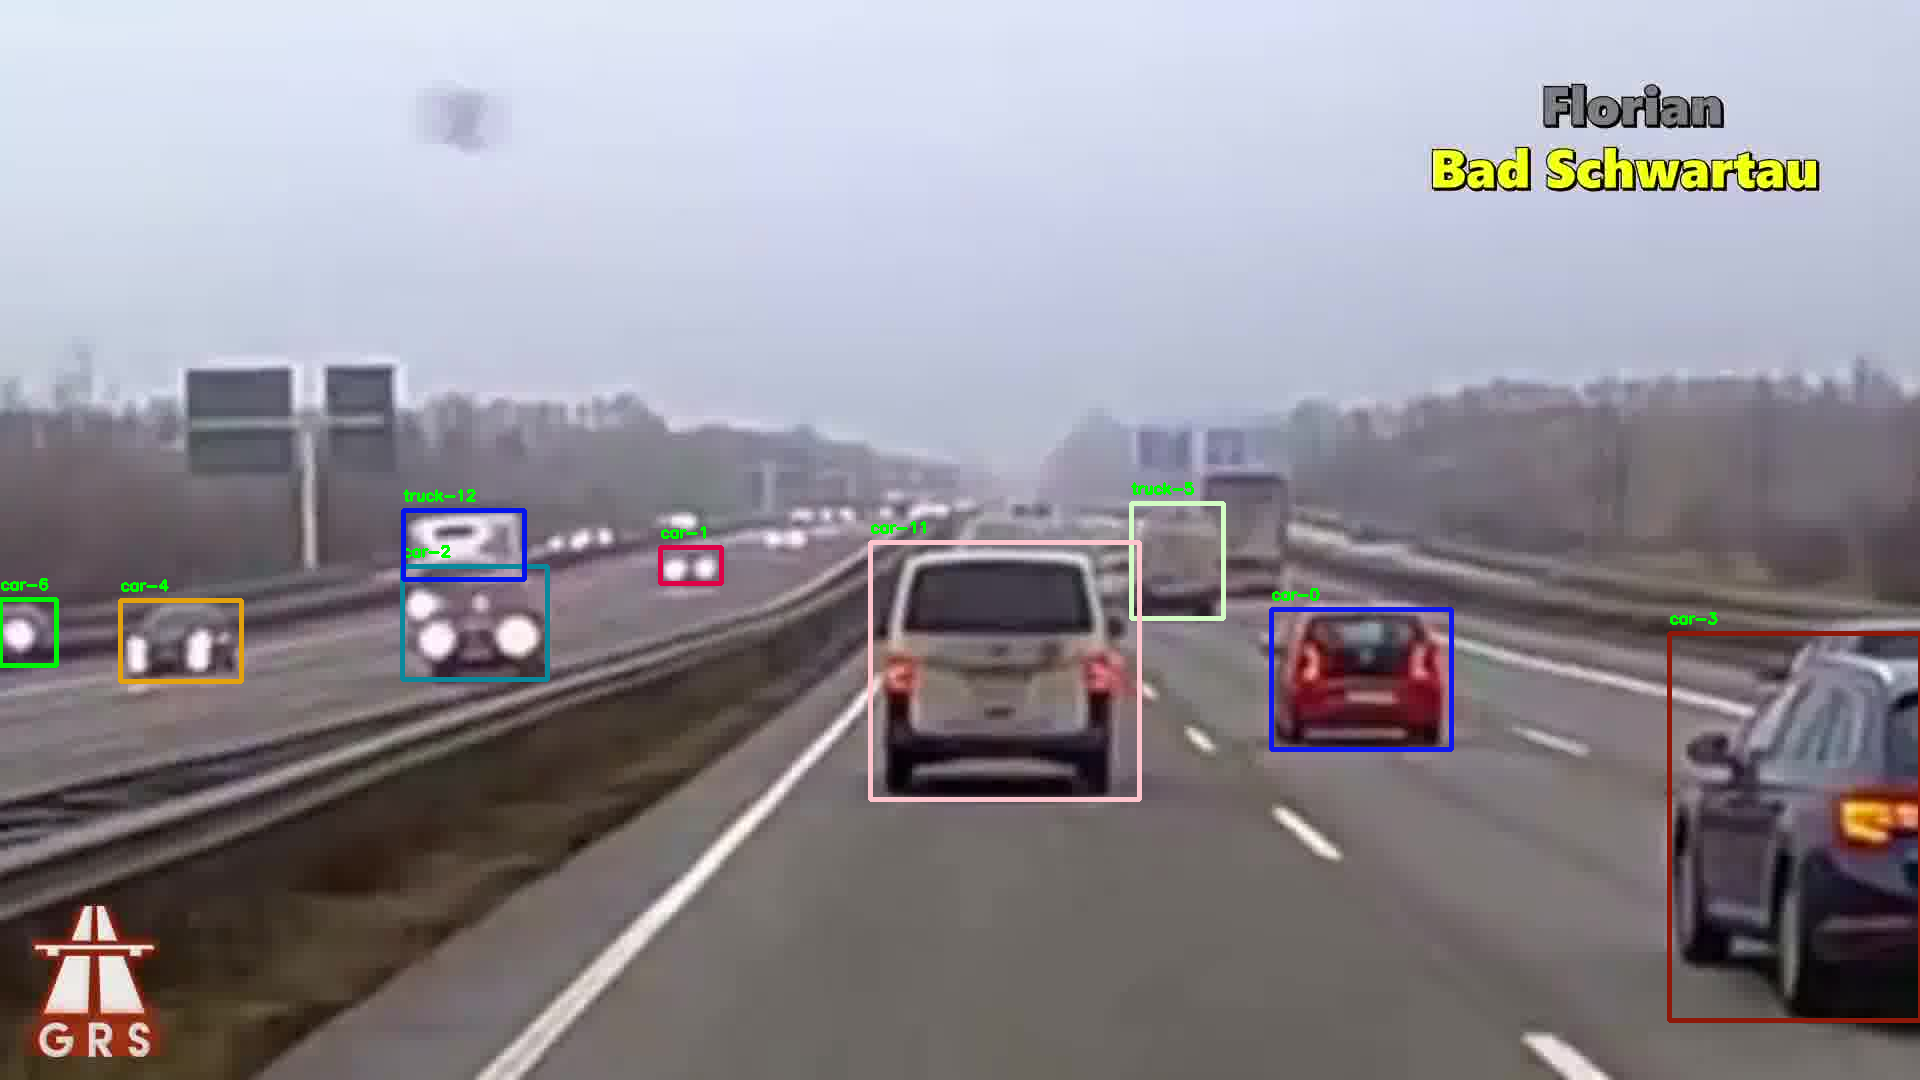
\includegraphics[width=\textwidth]{1}
\caption{\textit{frame start}}
\end{subfigure}
\label{fig:start_0}
\hfill
\begin{subfigure}[b]{0.48\textwidth}
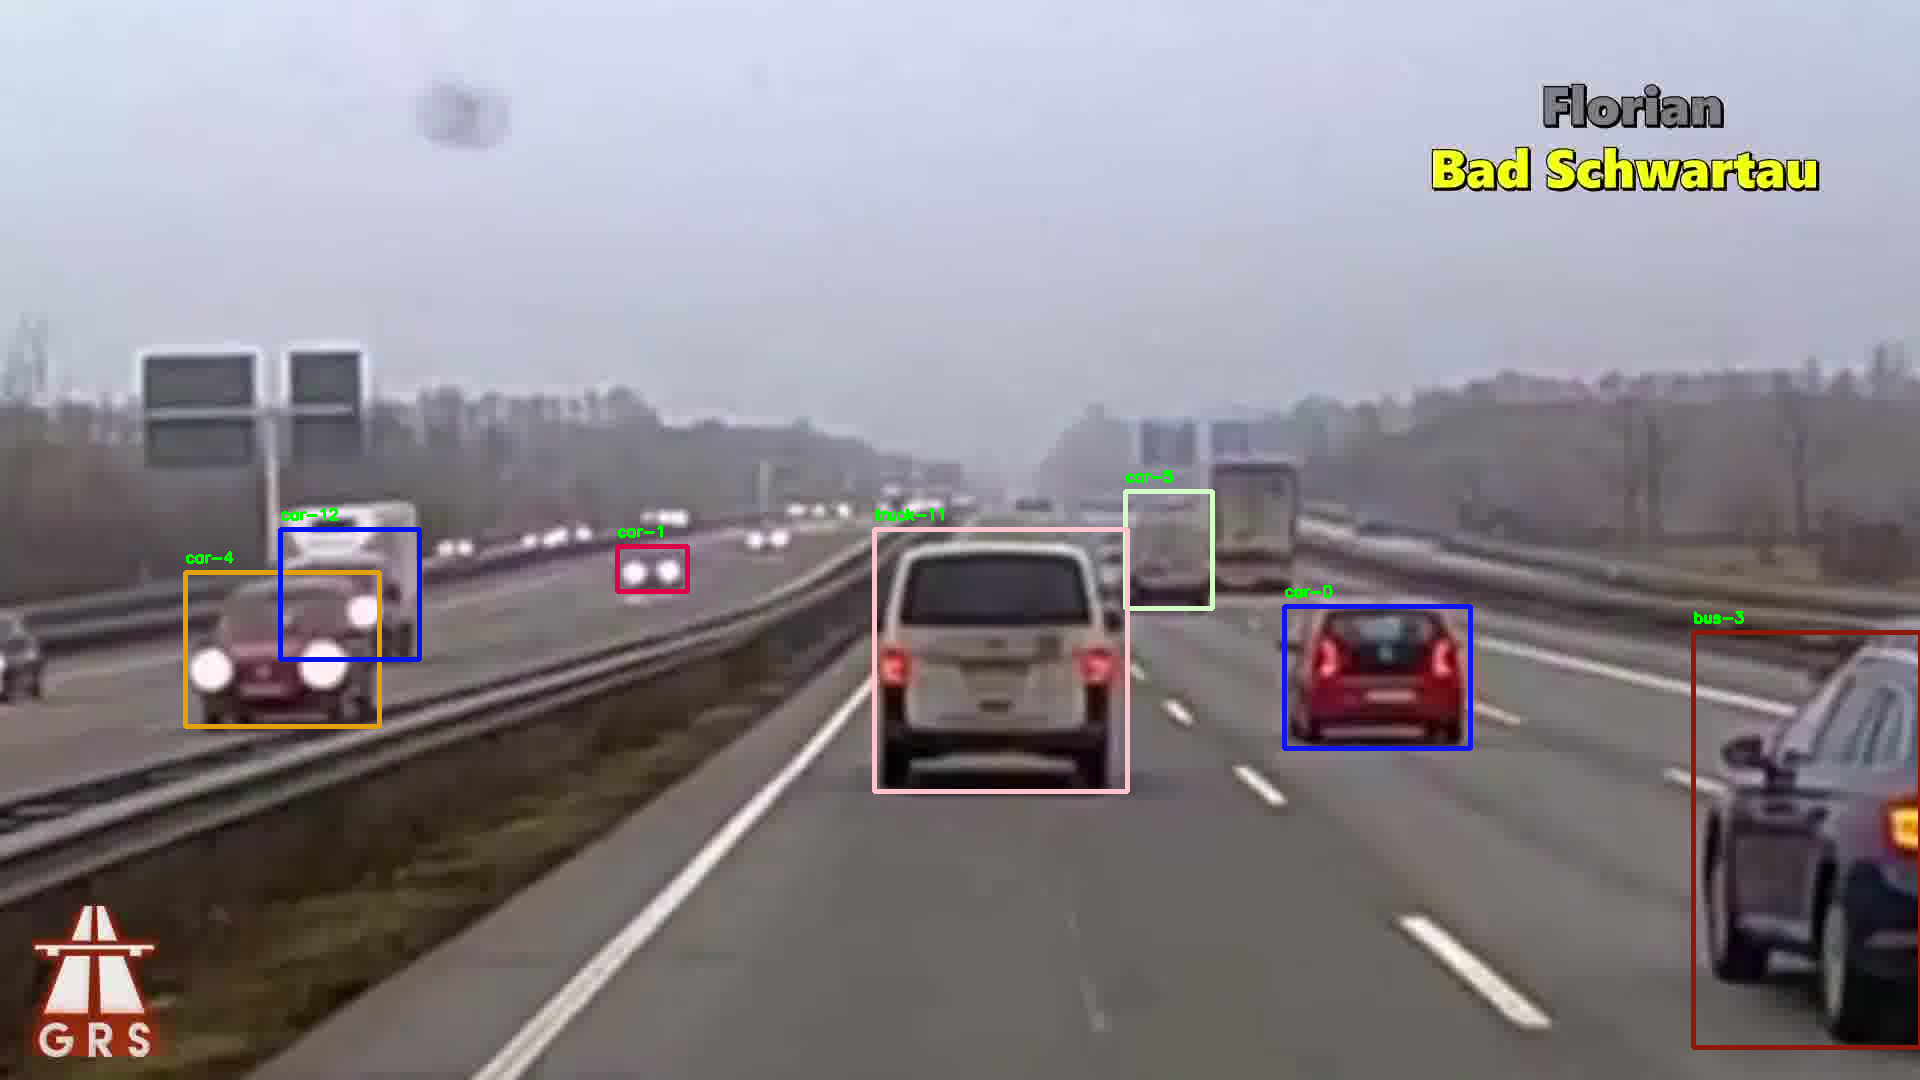
\includegraphics[width=\textwidth]{2}
\caption{\textit{frame start+1}}
\end{subfigure}
\label{fig:start_1}


\begin{subfigure}[b]{0.48\textwidth}
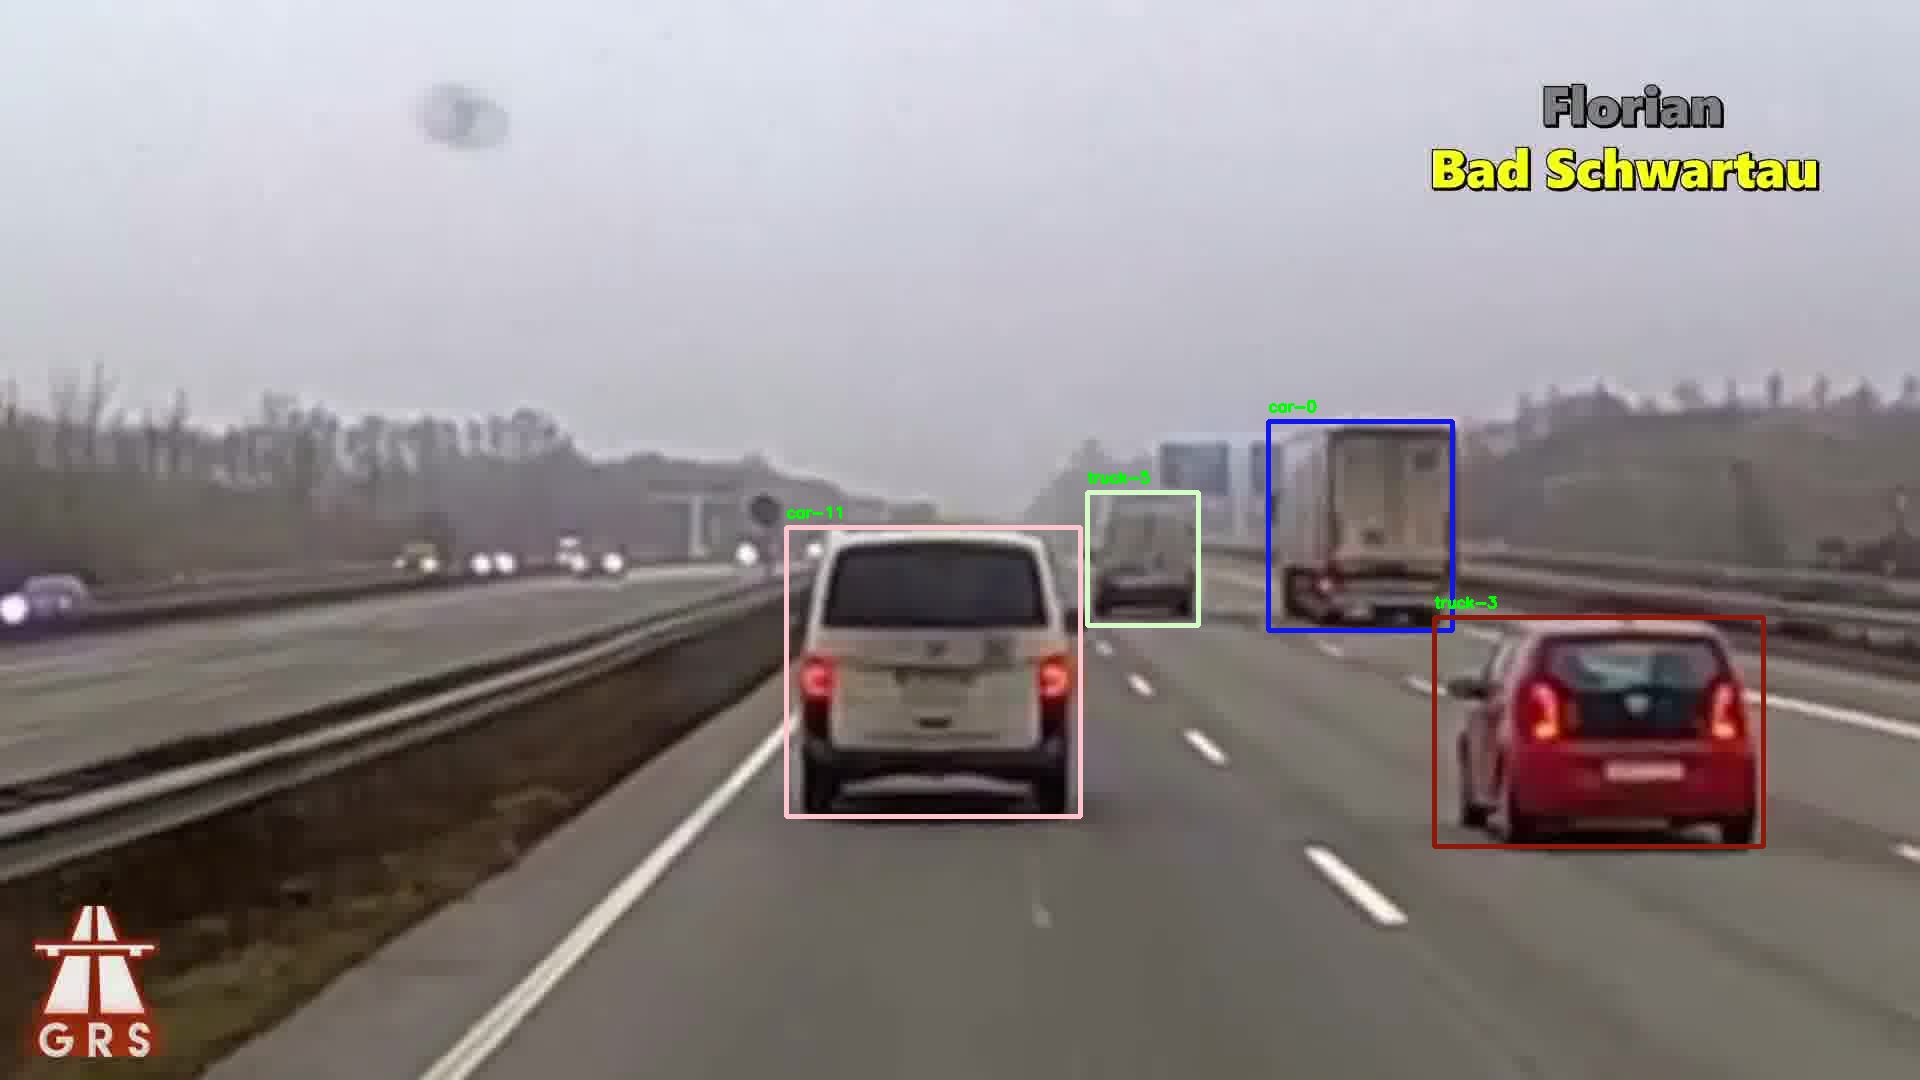
\includegraphics[width=\textwidth]{10}
\caption{\textit{frame middle}}
\end{subfigure}
\label{fig:middle_0}
\hfill
\begin{subfigure}[b]{0.48\textwidth}
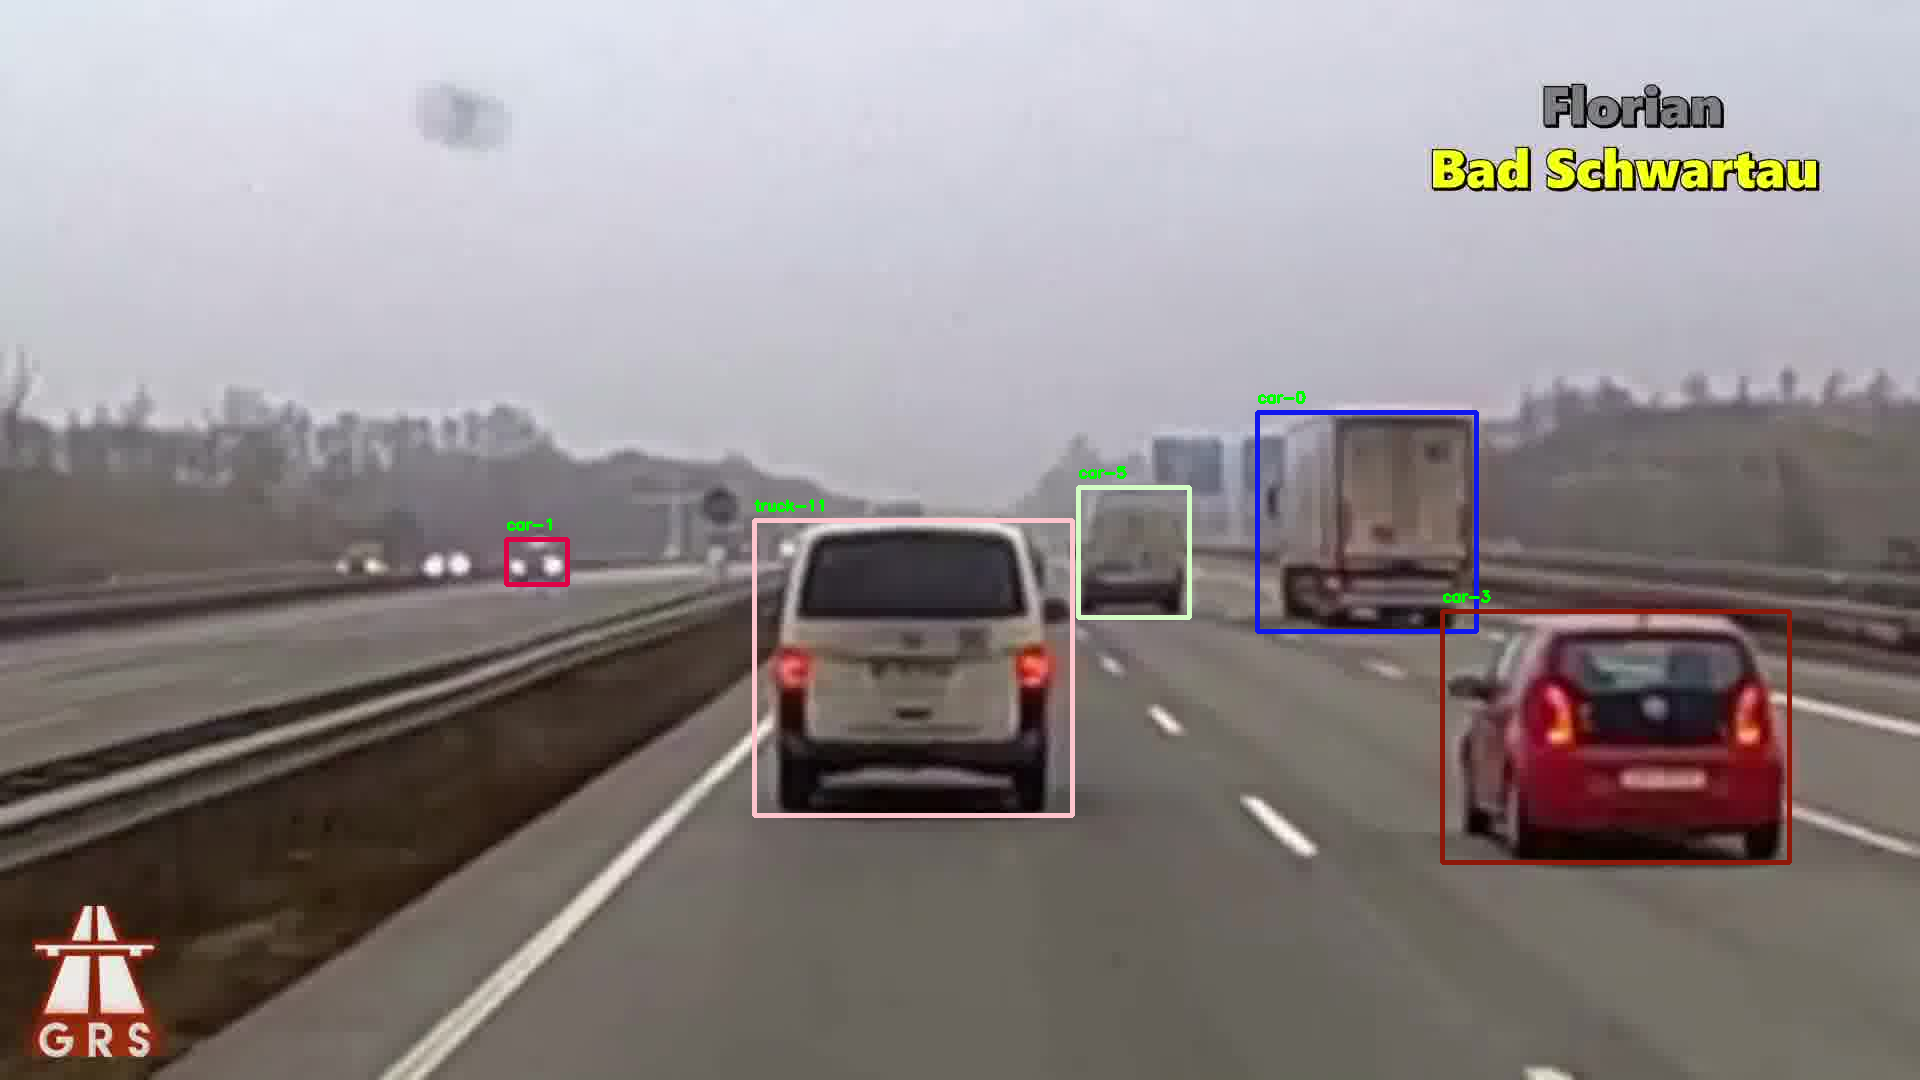
\includegraphics[width=\textwidth]{11}
\caption{\textit{frame middle+1}}
\end{subfigure}
\label{fig:middle_1}


\begin{subfigure}[b]{0.48\textwidth}
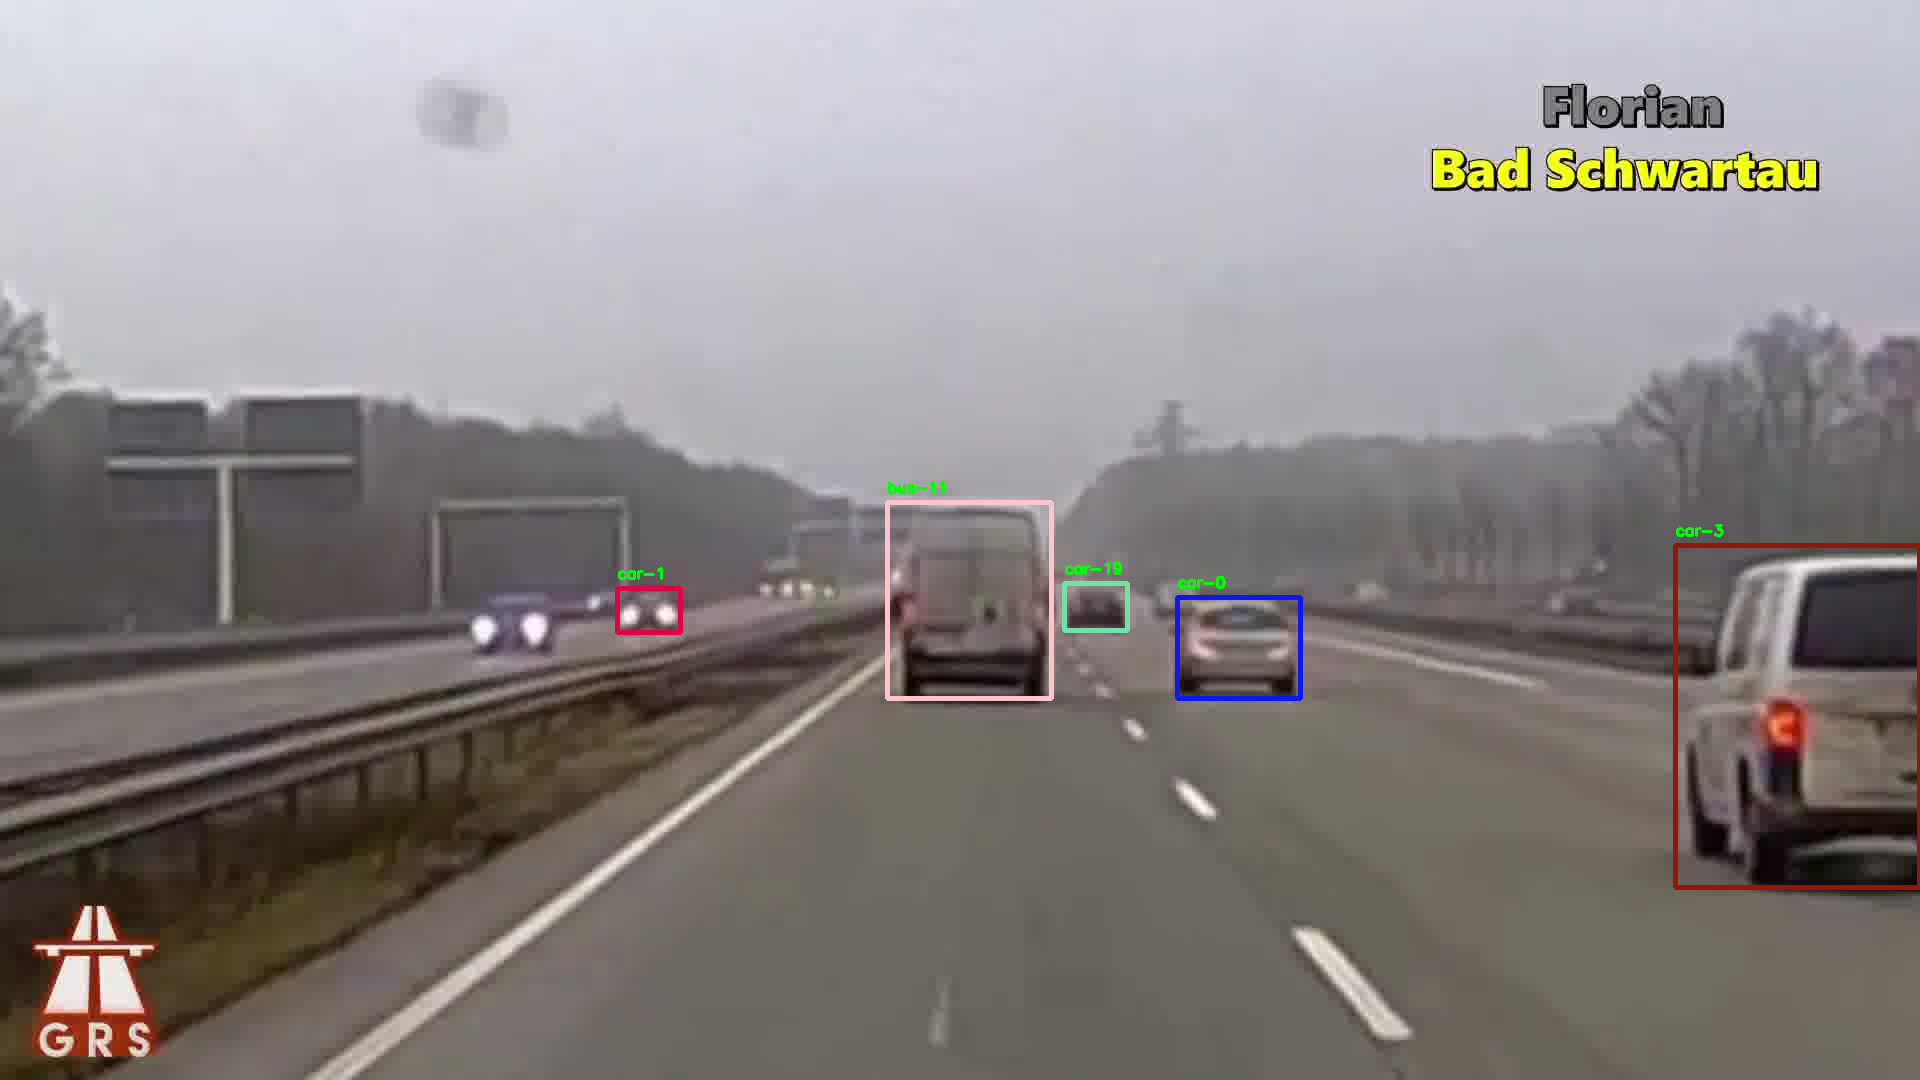
\includegraphics[width=\textwidth]{40}
\caption{\textit{frame 40}}
\end{subfigure}
\label{fig:end_0}
\hfill
\begin{subfigure}[b]{0.48\textwidth}
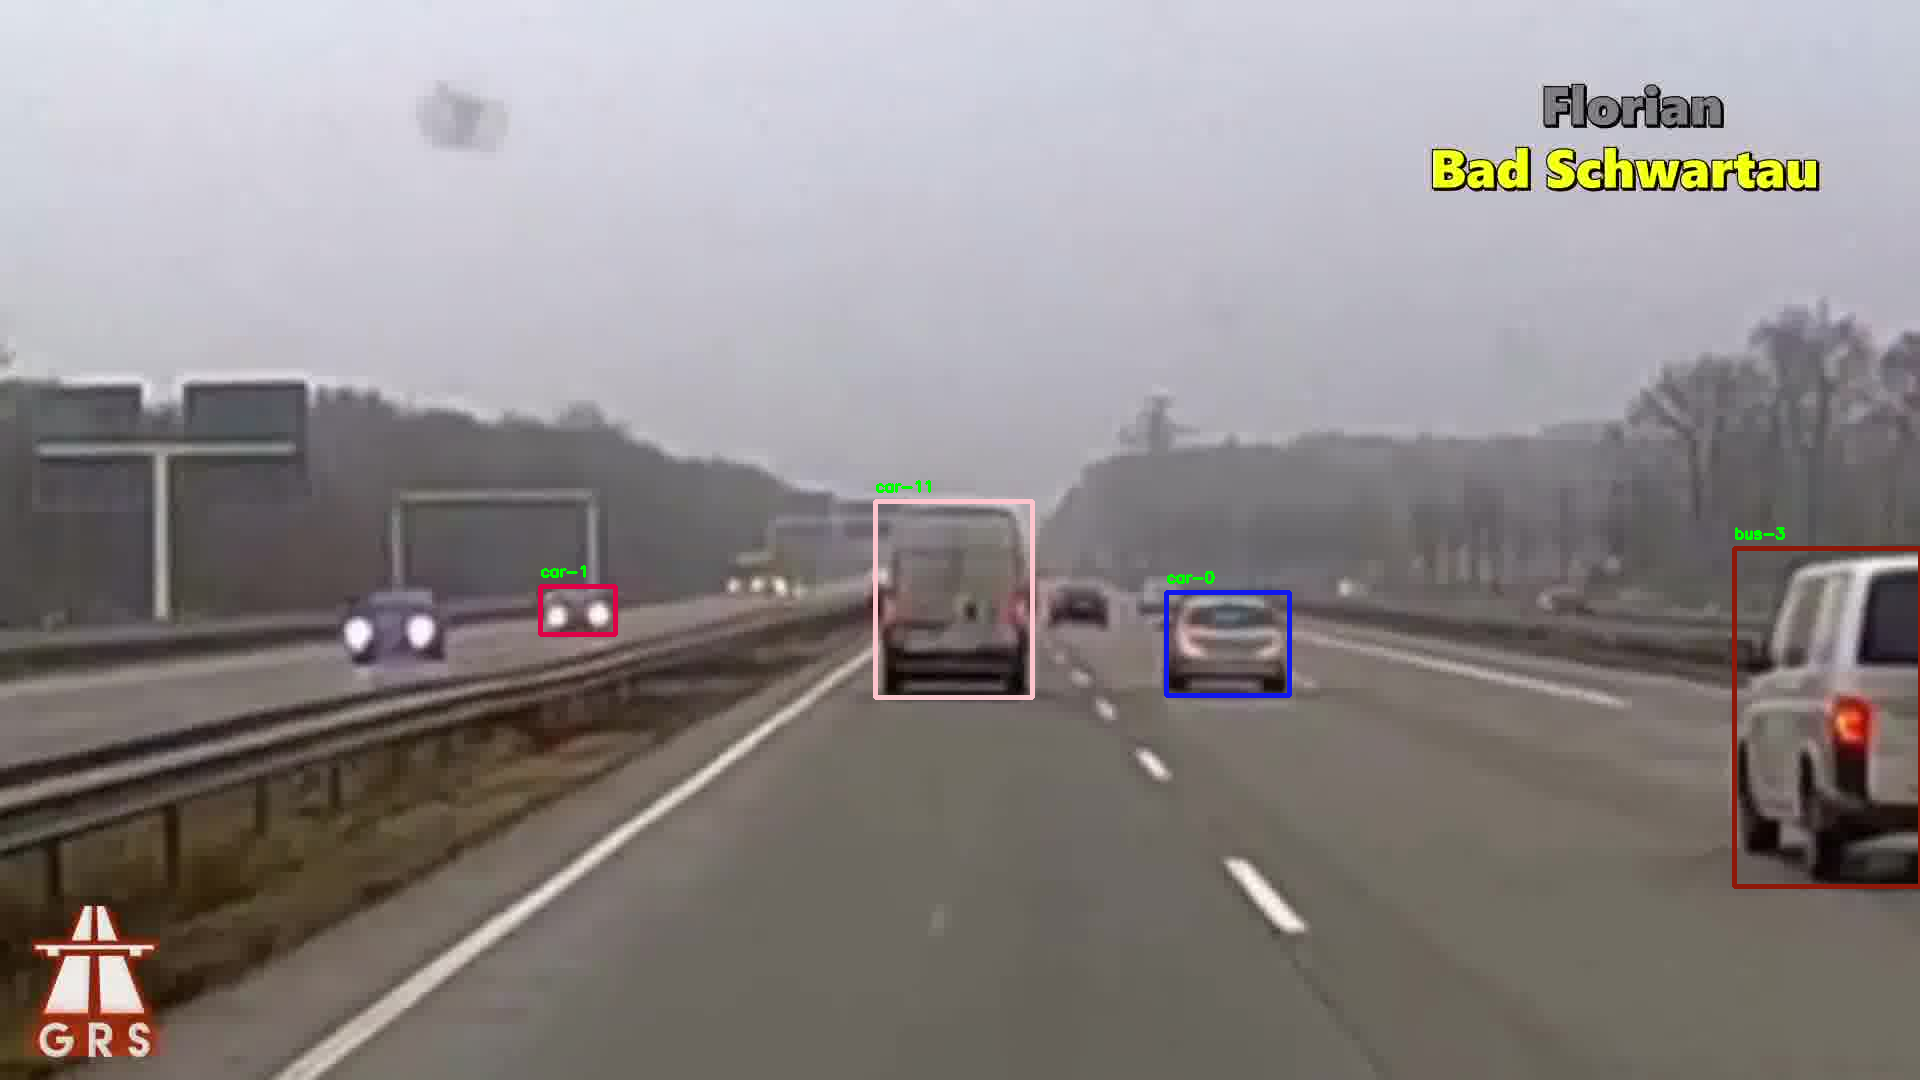
\includegraphics[width=\textwidth]{41}
\caption{\textit{frame 41}}
\end{subfigure}
\label{fig:end_1}
\caption{\textit{pairs visualization}}
\label{fig:tracked objects}
\end{figure}

 

\section{Algorithm} Tracking objects could be done via Intersection of Union or Euclidean distance. However, there is a problem of the IOU giving a  score of zero if there is no overlap between objects even if the tracked object moves a bit further from its original position. On the other hand, the Euclidean distance tends to calculate the minimum distance between the object in the previous frame and the current frame. Though both tracking strategies do not work with 100 $\%$ accuracy, the Euclidean distance turns to perform better. \\

\textbf{How the algorithm works}: 
\begin{itemize}
	\itemsep0em 
	\item The euclidean distance between the current boxes and previous boxes are calculated. 
	\item For each object in the current frame an object with minimum euclidean distance from the previous frame is chosen.
	\item Track ID and COLOR are used for tracking.
	\item Register new objects if they have not been seen before.
	\item Deregister the object that disappears after one frame, and register it as a new object if it appears again. 
\end{itemize}

The baseline model (i.e. Detectron model) is able to detect an object in a frame but sometimes is unable to detect that same object in a different frame. Therefore, improvement in the Detectron model will highly improve the Euclidean distance algorithm as well. In cases the Detectron is unable to detect similar objects in different frames, the tracking algorithm de-register that particular object and registers it again if it reappears. This issue, therefore, can be resolved by setting a "maxDisappearance" variable and this value should be greater than 0. However, this is not an efficient method because the bounding box plot will sometimes get stuck on the previous frame even if the objects disappear. Aside from this, maxDisappearance  of 0 works so well most of the time.\\

\begin{figure*}[ht!]
	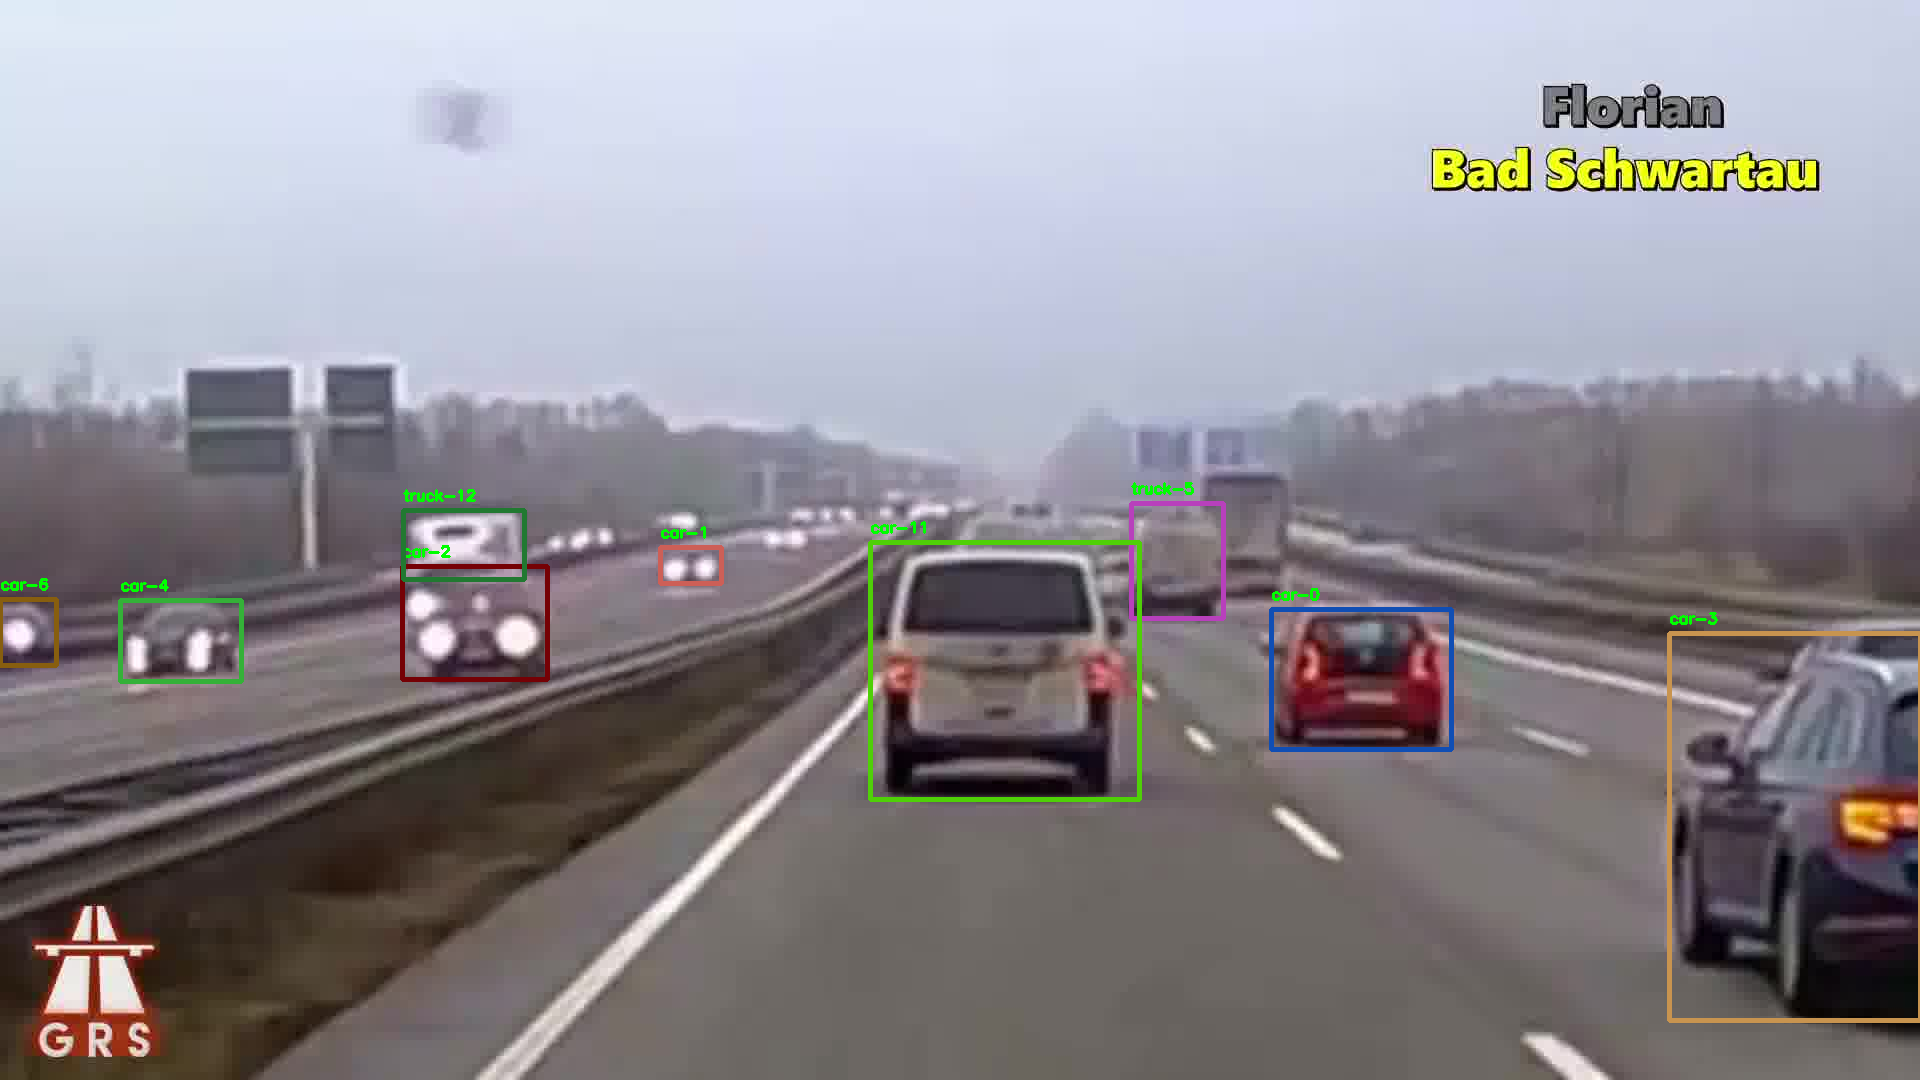
\includegraphics[width=.3\textwidth]{f1}\hfill
	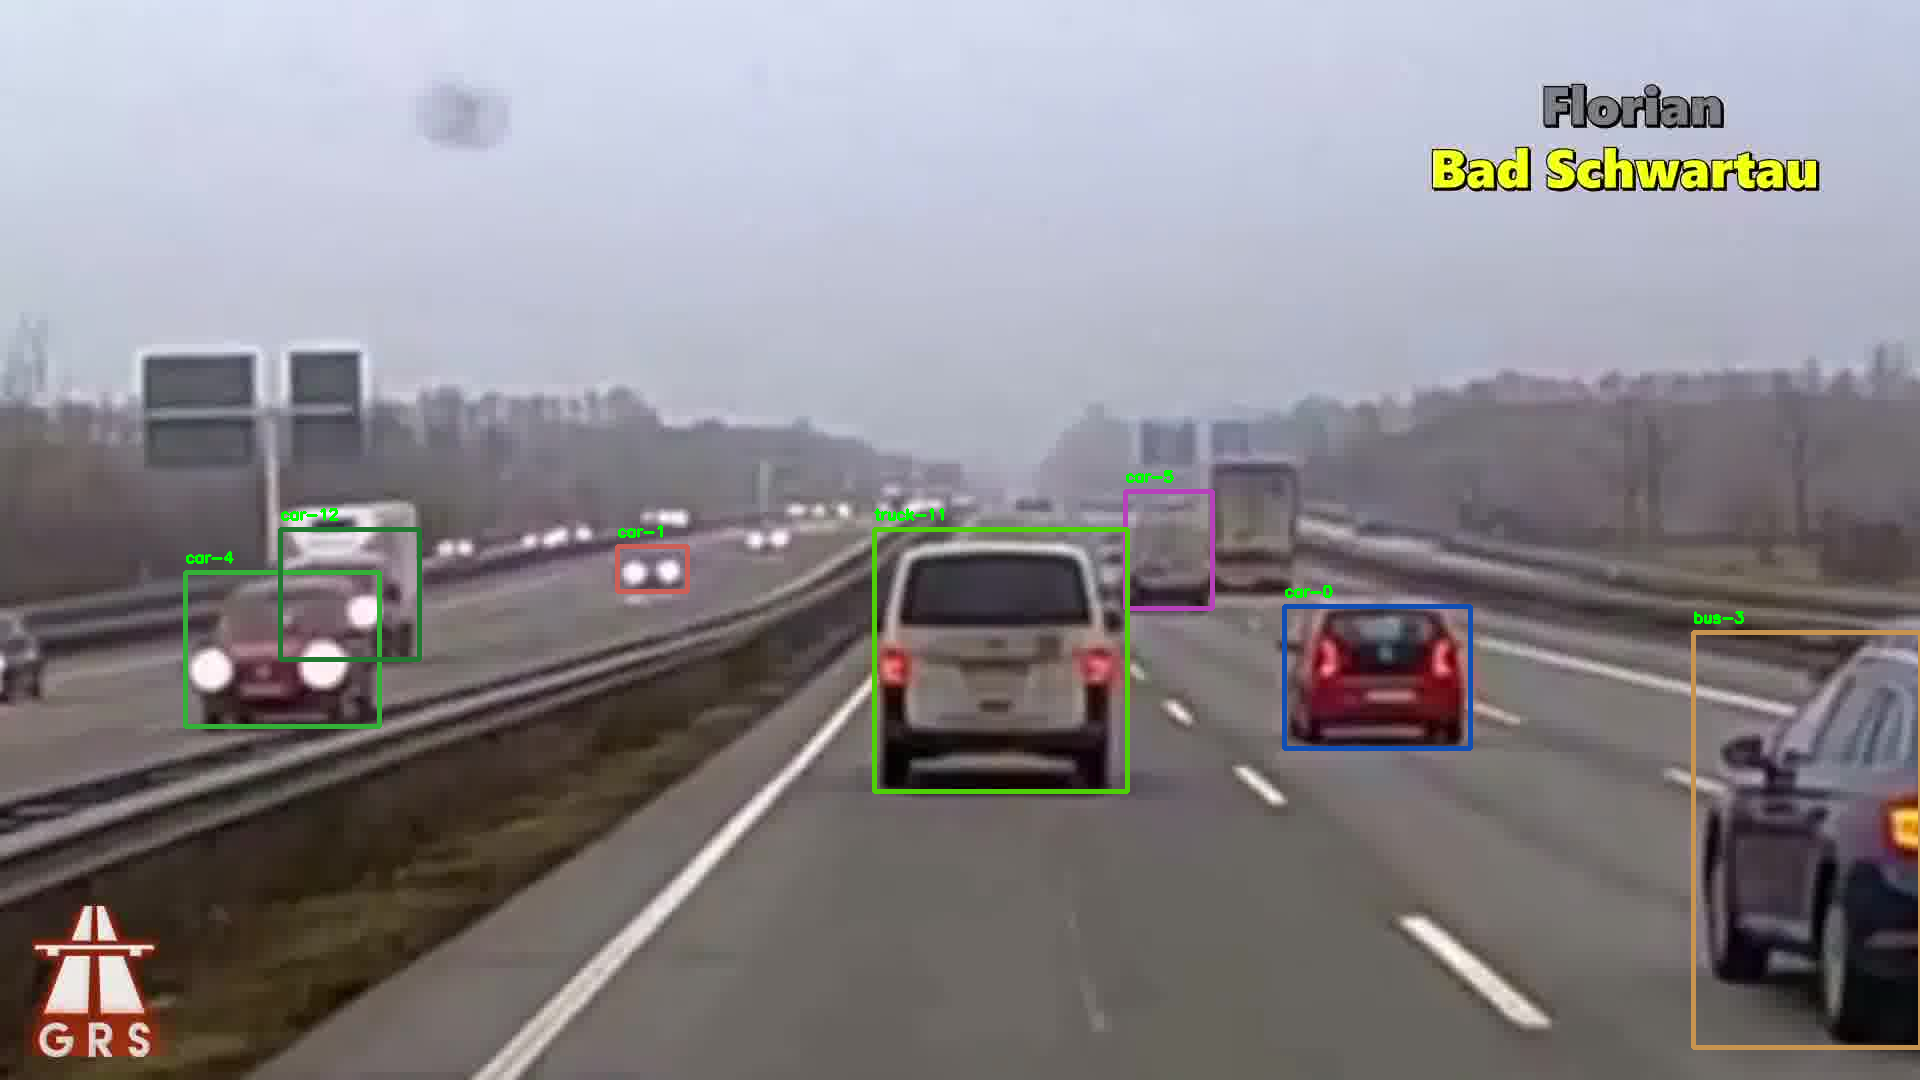
\includegraphics[width=.3\textwidth]{f2}\hfill
	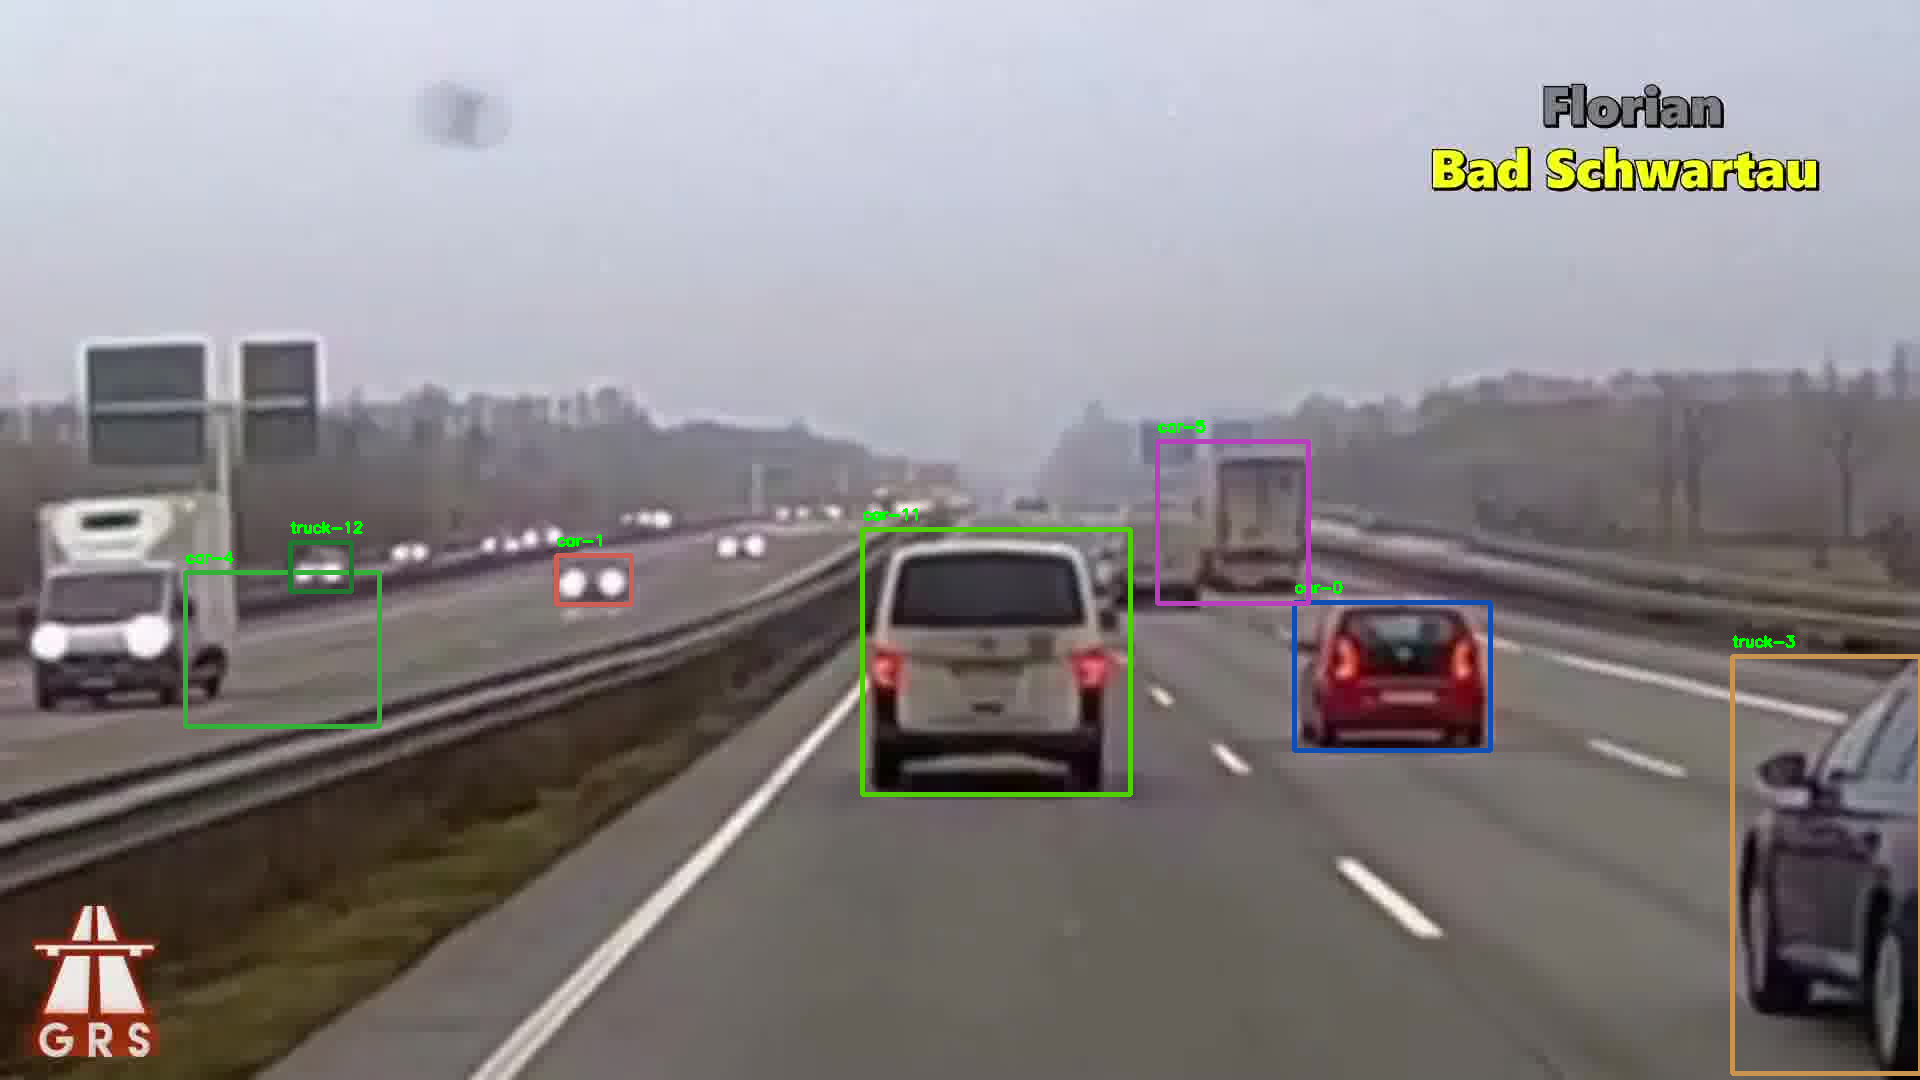
\includegraphics[width=.3\textwidth]{f3}\hfill
	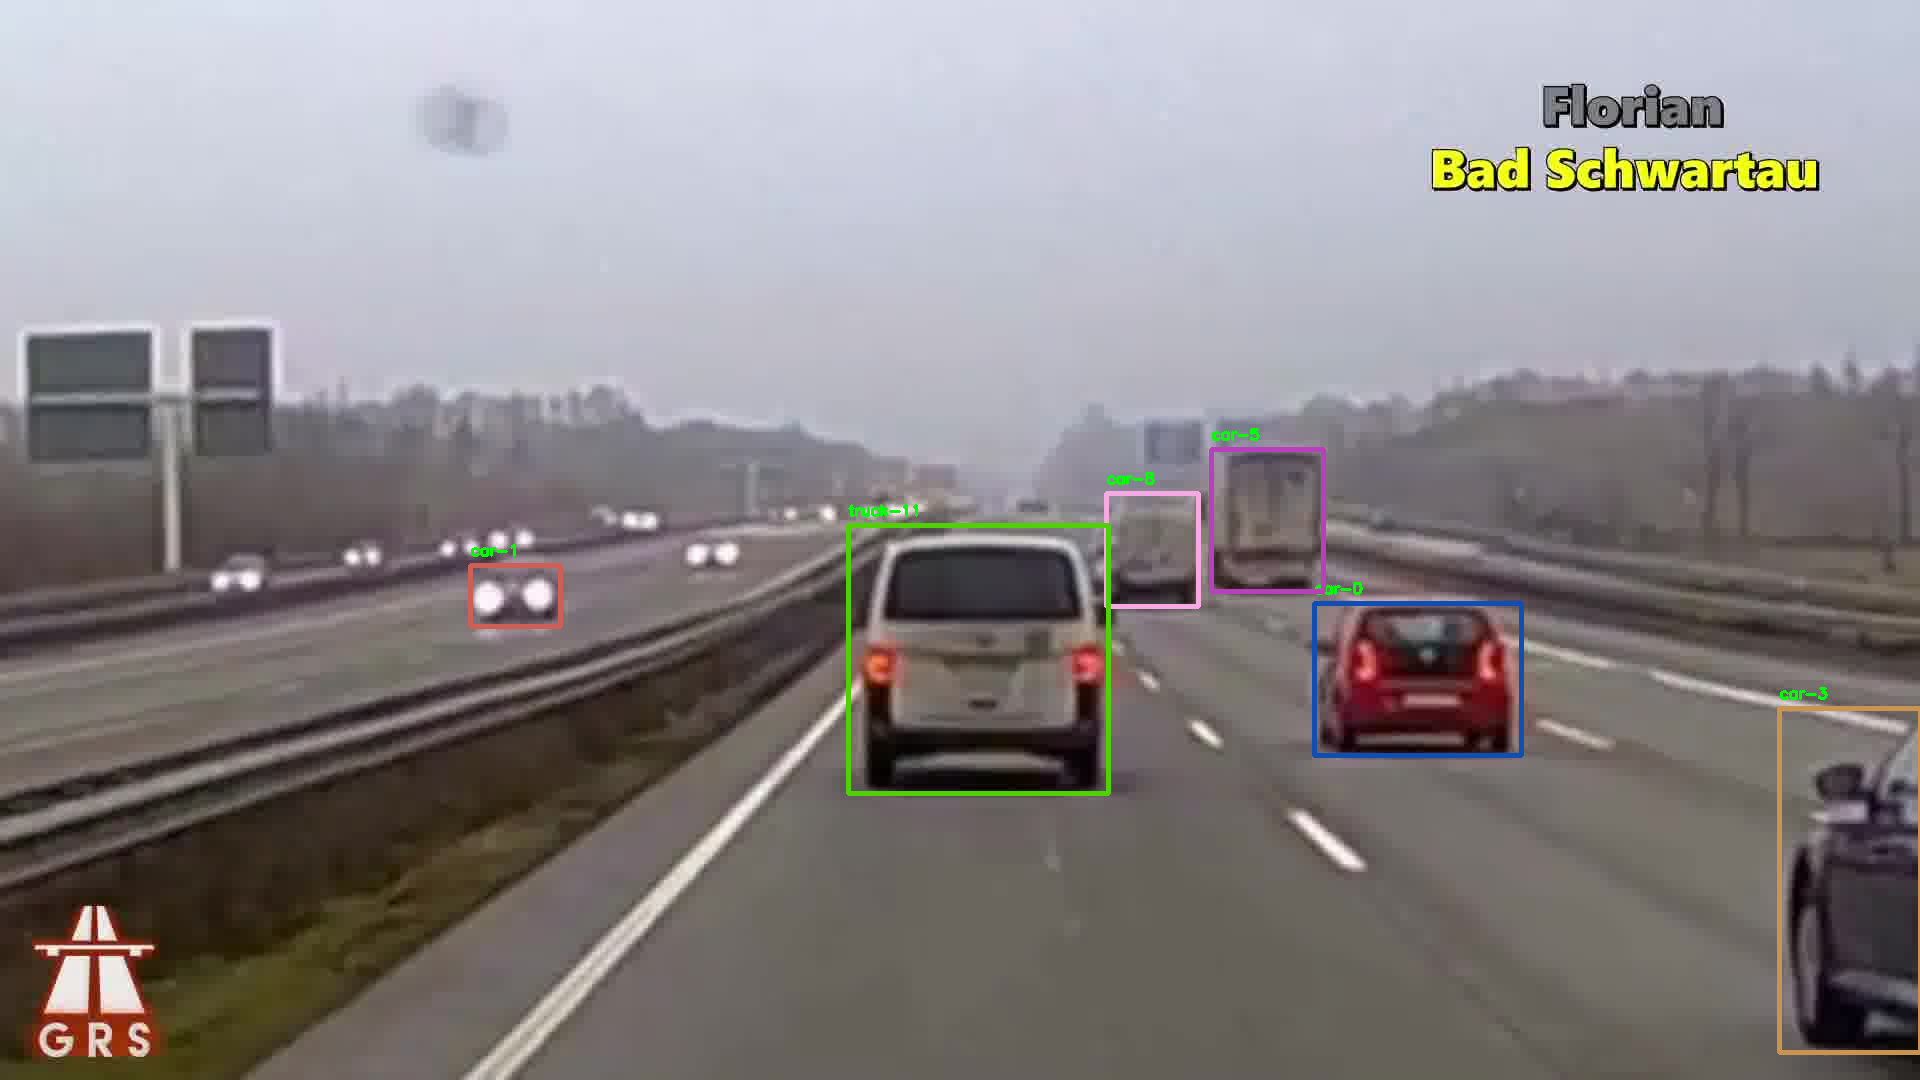
\includegraphics[width=.3\textwidth]{f4}\hfill
	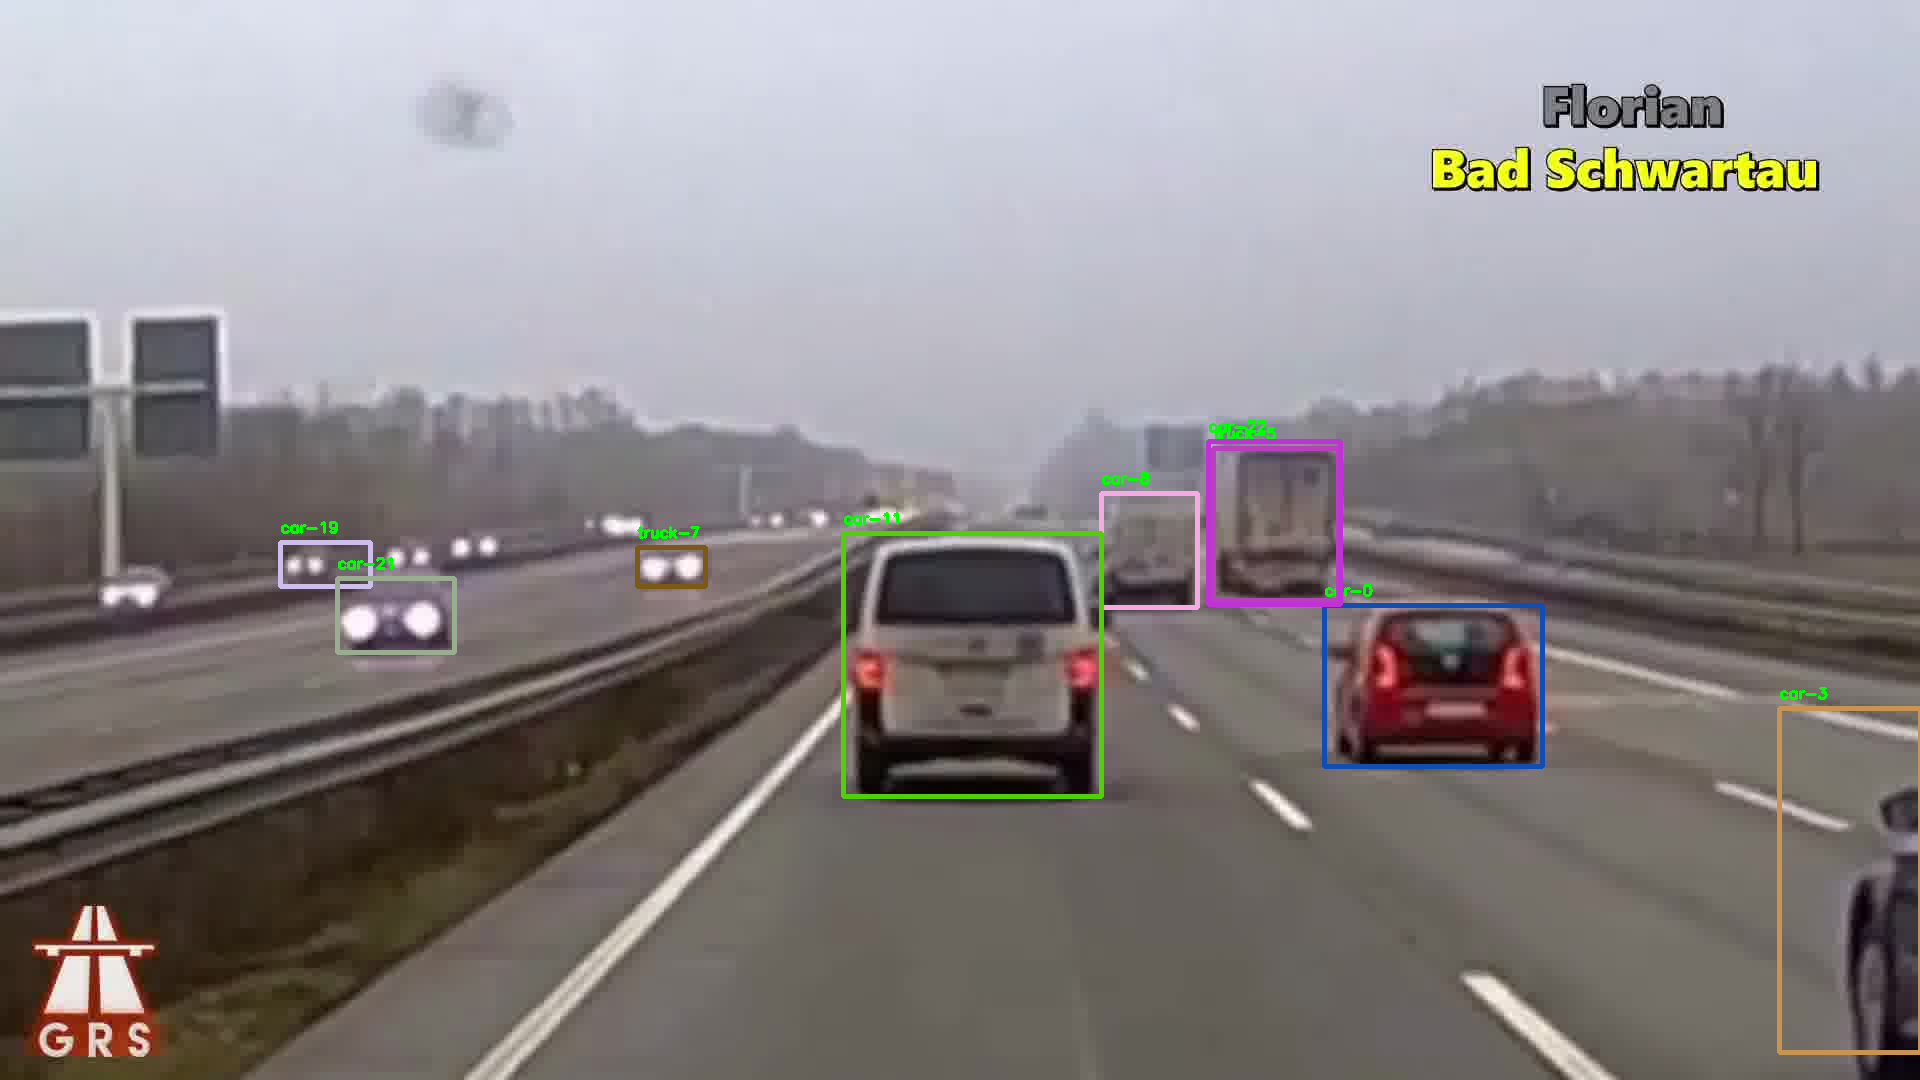
\includegraphics[width=.3\textwidth]{f5}\hfill
	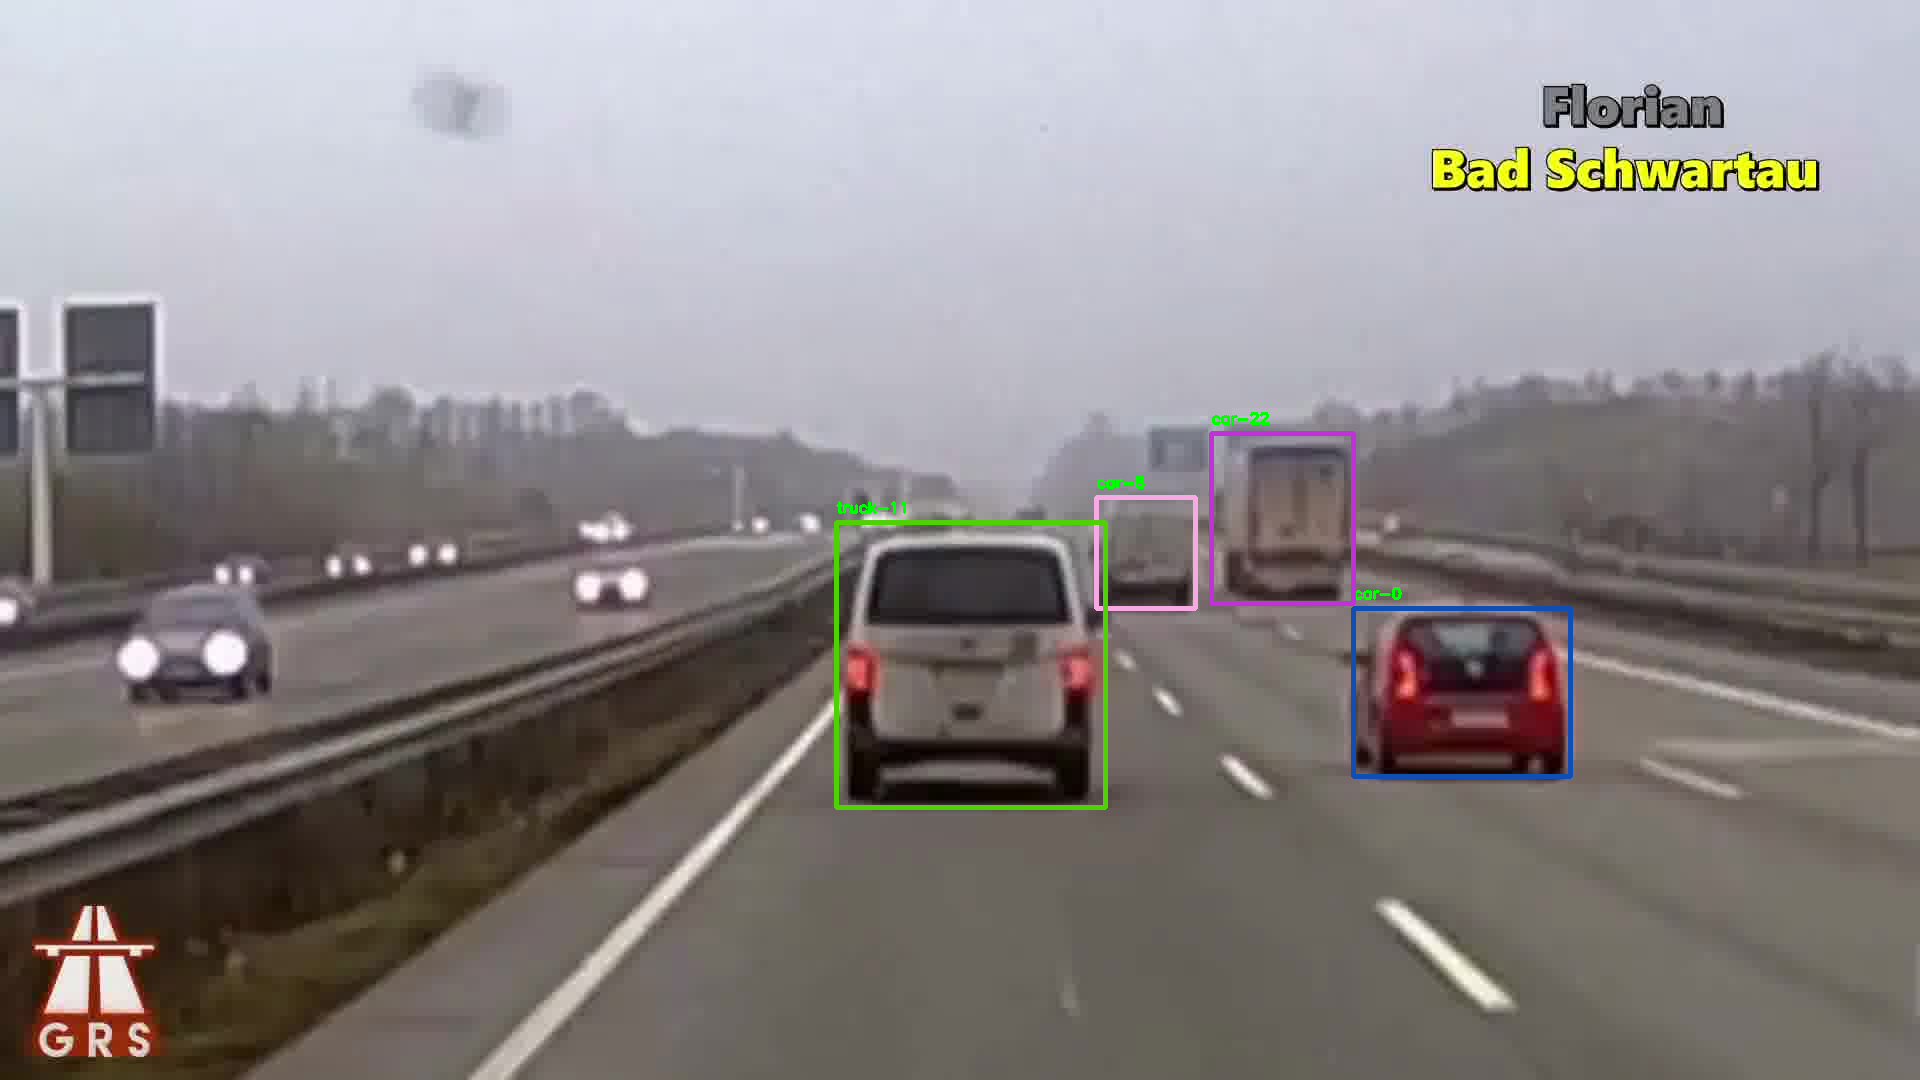
\includegraphics[width=.3\textwidth]{f6}\hfill
	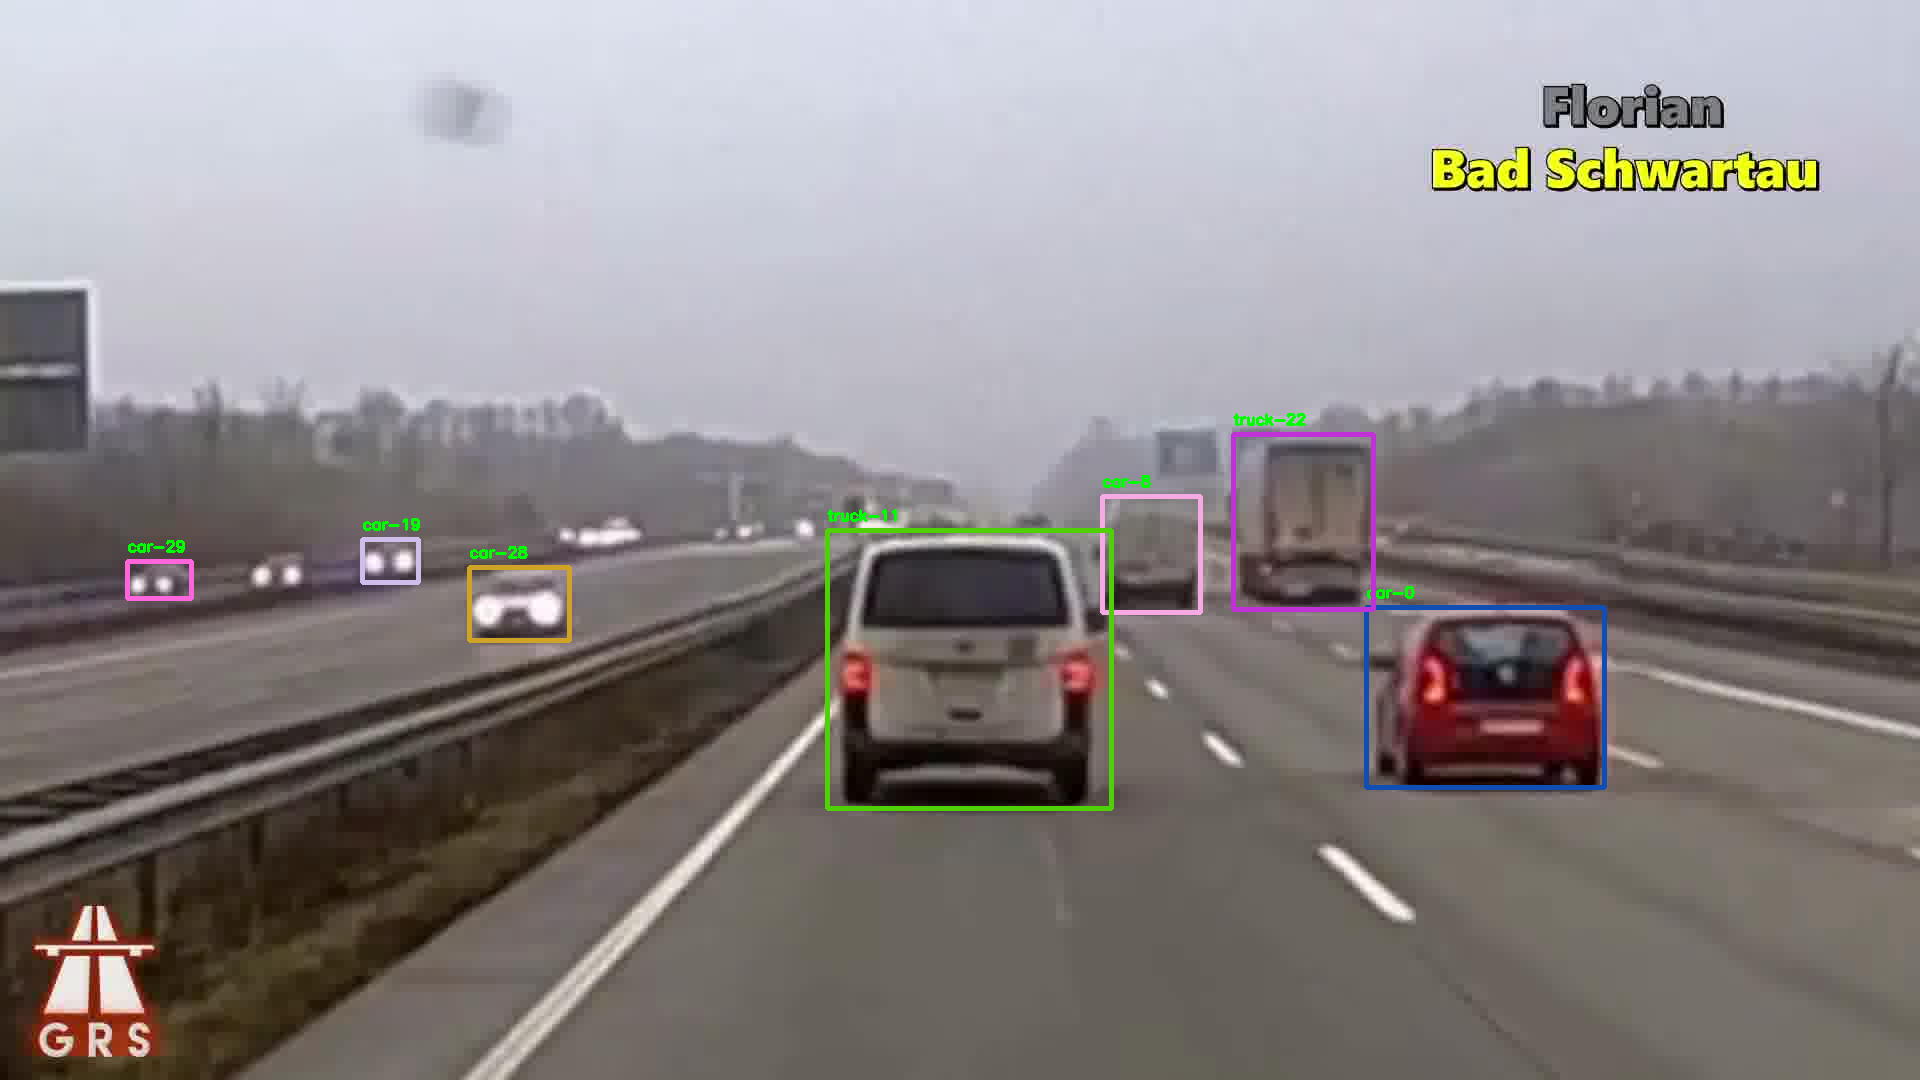
\includegraphics[width=.3\textwidth]{f7}\hfill
	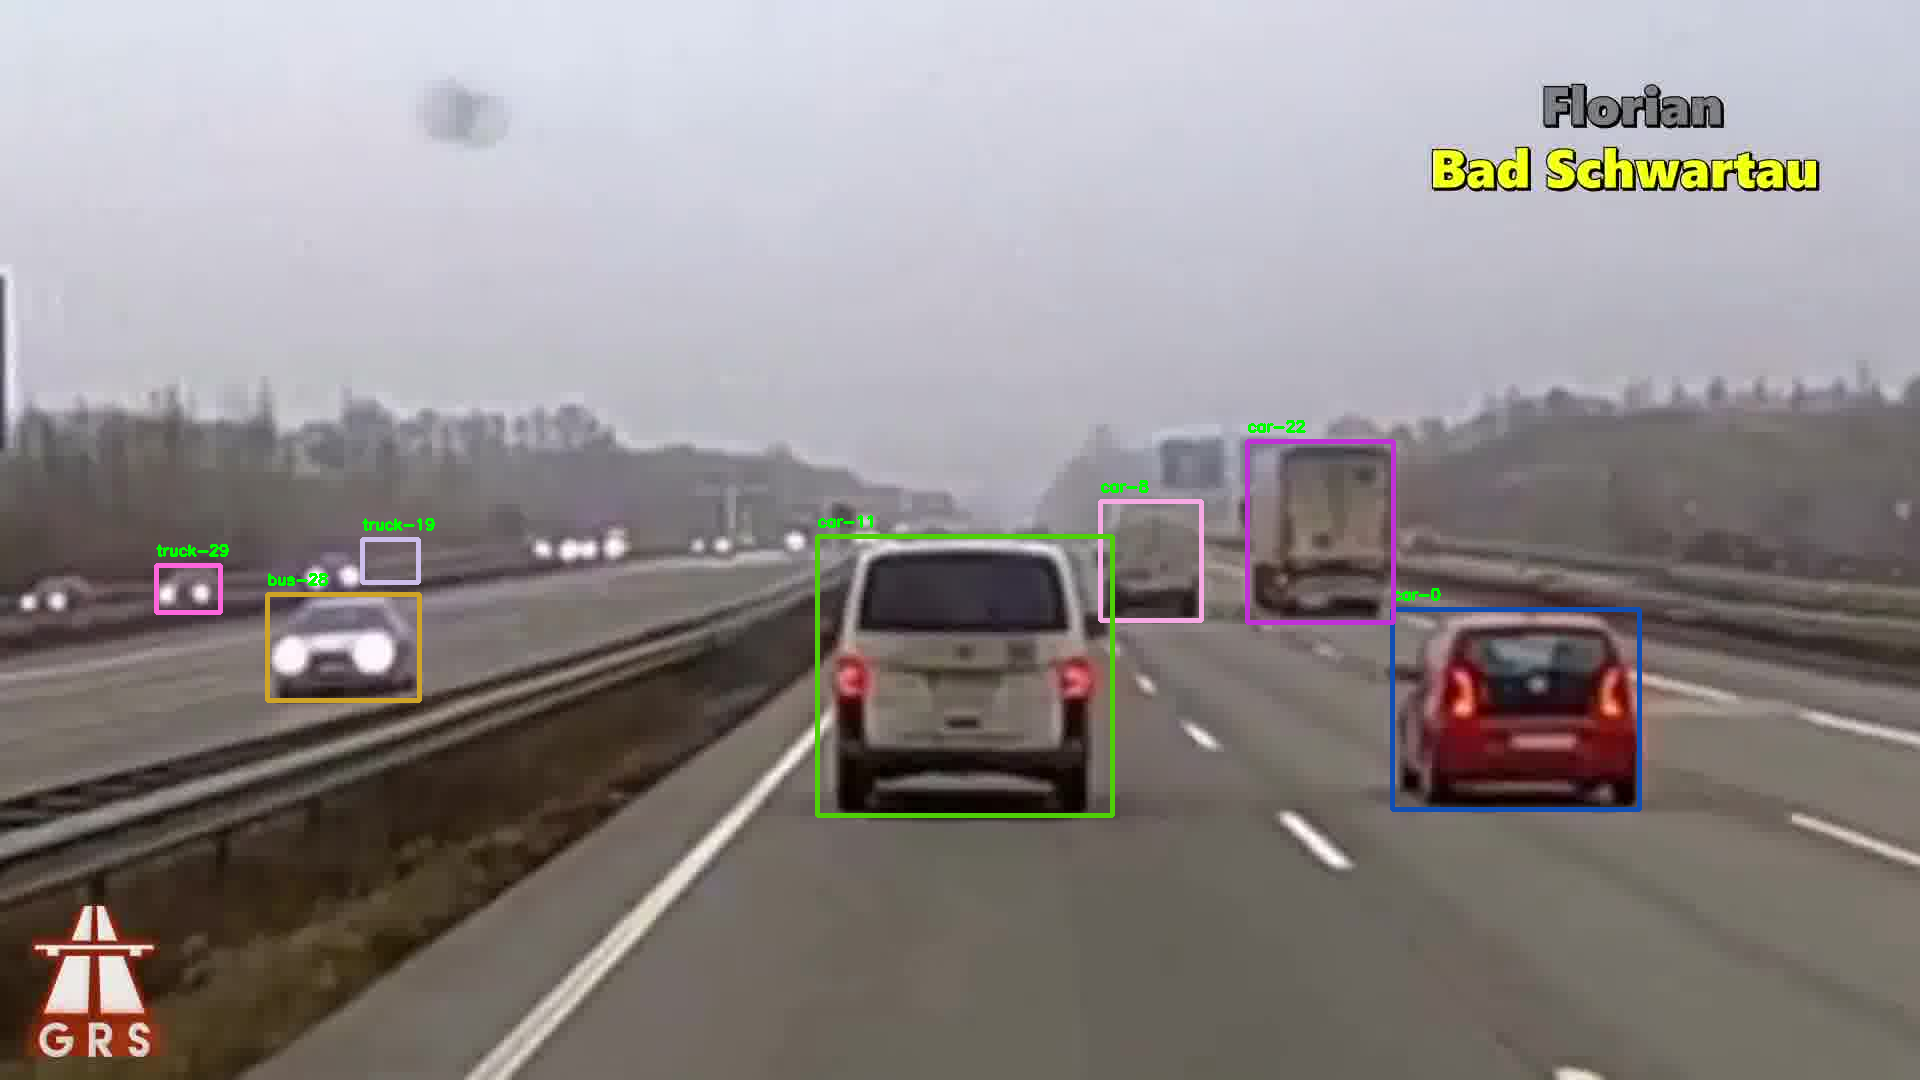
\includegraphics[width=.3\textwidth]{f8}\hfill
	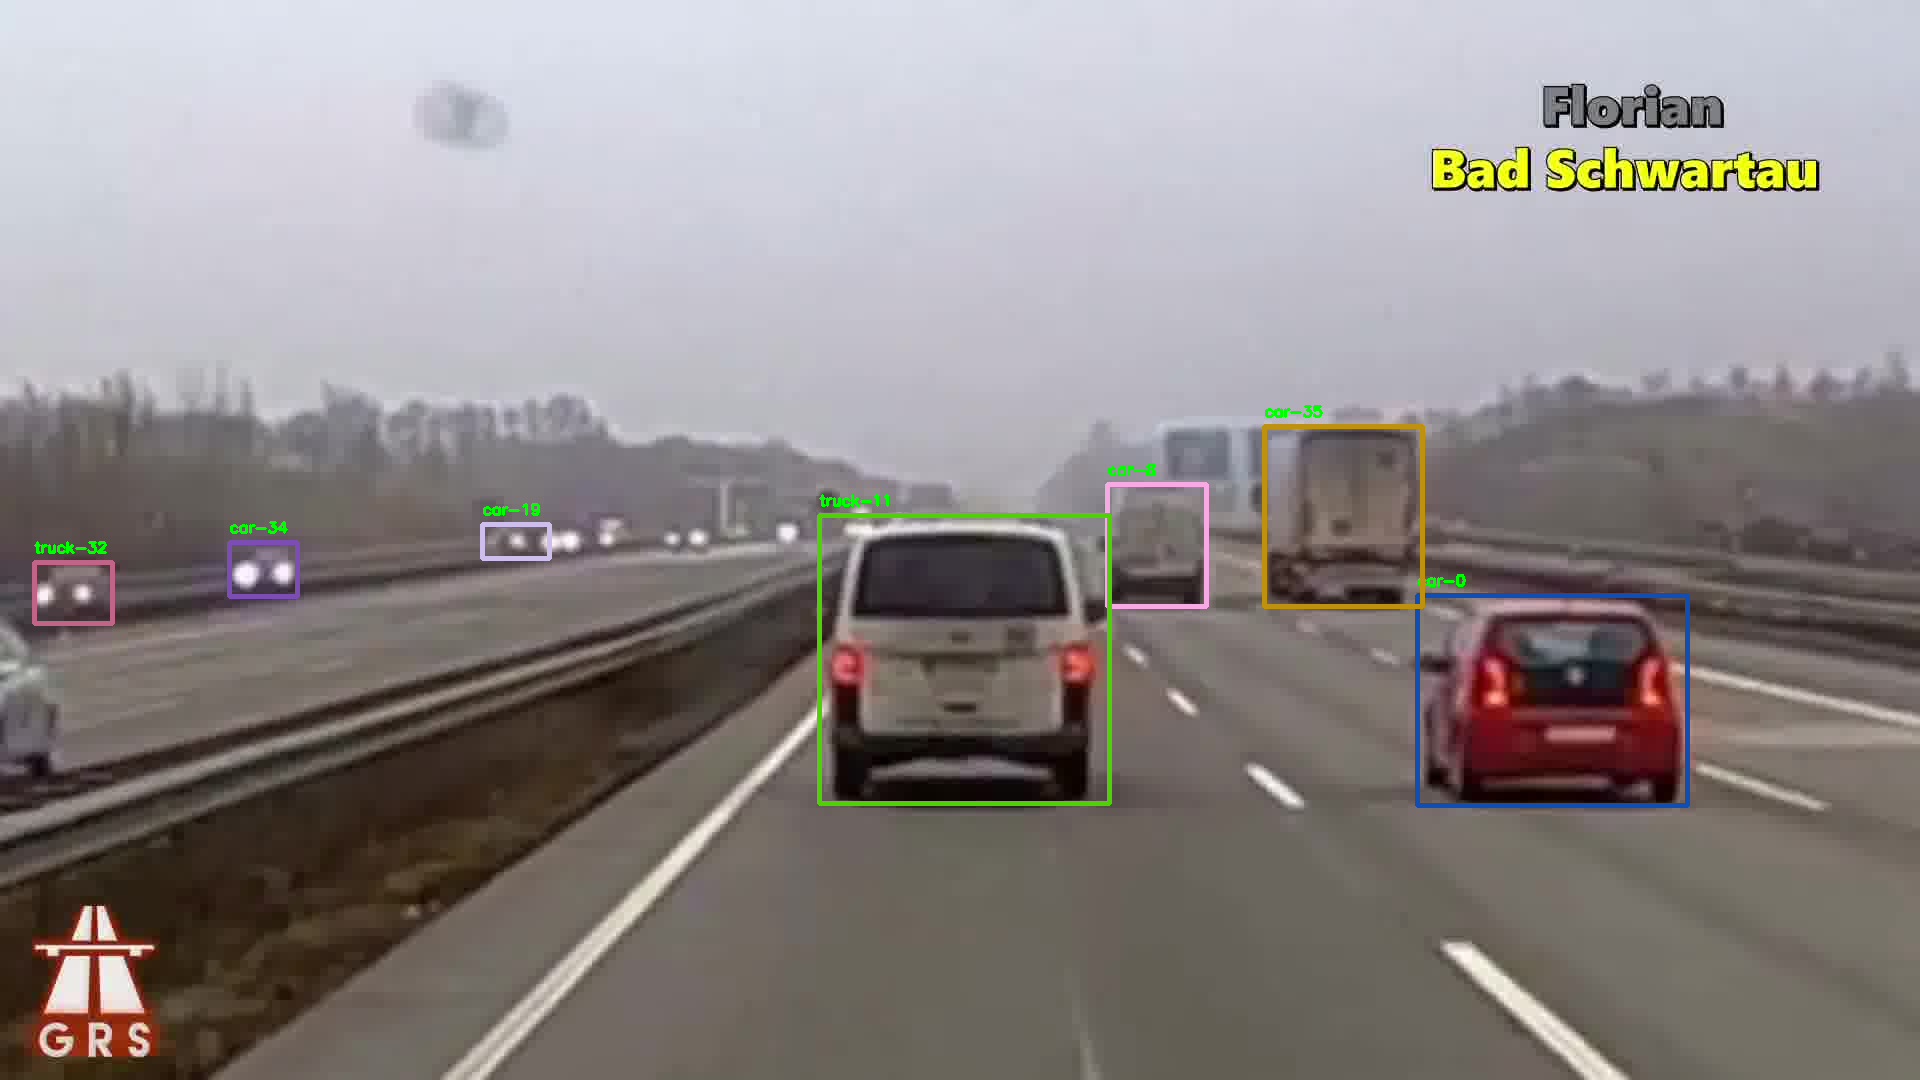
\includegraphics[width=.3\textwidth]{f9}\hfill
	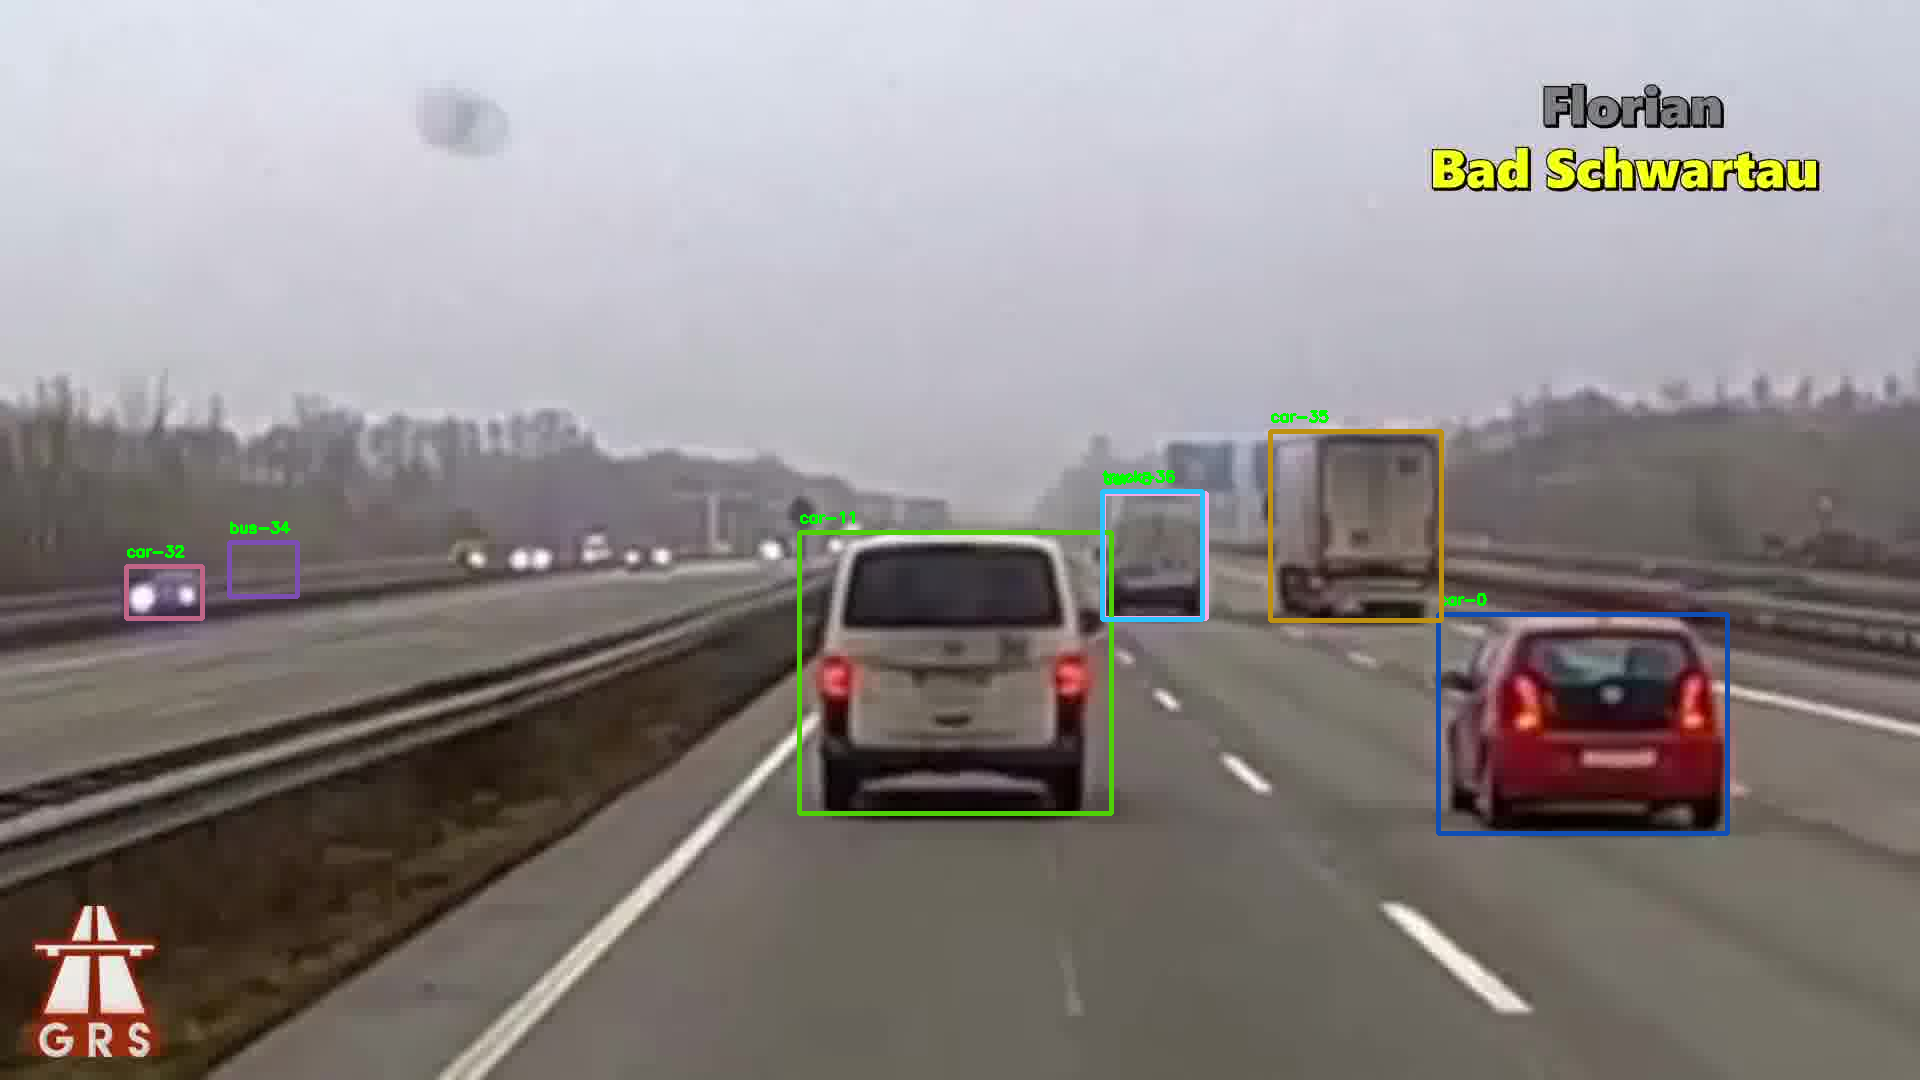
\includegraphics[width=.3\textwidth]{f10}\hfill
	\caption{$10$ consecutive frames from the video}
	\label{fig:vid10}
\end{figure*}


\section{Visualizations}
Figure \ref{fig:tracked objects} demonstrates a pair of objects from different locations of the video. Similarly, figure \ref{fig:vid10} shows 10 consecutive frames from the video. as can be seen from the color and the track ID, we can say that the algorithm is doing well on tracking the objects shown. Also, you can find here \href{https://drive.google.com/file/d/1SU9l7xqWIhSBf2u6otgfuCLeYygQN1v6/view?usp=sharing}{link} a video for all the frames. As can be seen from the video, when color changes after sequence of frames, it is due to detectron's different prediction of the same object or detectron did not detect that object in one of the frames.  Similarly, there sometimes exist a lot of overlapping objects, but luckily, thresholding based on detectron's prediction score and box area is used to alleviate  this issue. Overall, the algorithm is working quite well with mimumum configuration in all frames. 

\section{Conclusion}
Tracking objects in a video or live stream is a challenging problem, particularly when the speed of objects is so fast, or objects have occluded each other. In this lab we showed how euclidean distance helps in tracking objects in video. Finally, I can conclude that The project was fascinating, and I have learned a lot in object tracking. 

\end{document}\\